%%%%%%%%%%%%%%%%%%%%%%%%%%%%%%%%%%%%%%%%%%%%%%%%%%%%%%%%%%%%%%%%%%%%%%%%%%%%%%%%
%2345678901234567890123456789012345678901234567890123456789012345678901234567890
%        1         2         3         4         5         6         7         8

%\documentclass[journal,transmag]{IEEEtran}% Comment this line out if you need a4paper

\documentclass[10pt, conference]{ieeeconf}      % Use this line for a4 paper

\IEEEoverridecommandlockouts                              % This command is only needed if 
                                                          % you want to use the \thanks command

%\overrideIEEEmargins                                      % Needed to meet printer requirements.

% See the \addtolength command later in the file to balance the column lengths
% on the last page of the document

% The following packages can be found on http:\\www.ctan.org
%\usepackage{graphics} % for pdf, bitmapped graphics files
%\usepackage{epsfig} % for postscript graphics files
%\usepackage{mathptmx} % assumes new font selection scheme installed
%\usepackage{times} % assumes new font selection scheme installed
%\usepackage{amsmath} % assumes amsmath package installed
%\usepackage{amssymb}  % assumes amsmath package installed

\newtheorem{theorem}{Theorem}[section]
\newtheorem{lemma}[theorem]{Lemma}
\newtheorem{proposition}[theorem]{Proposition}
\newtheorem{corollary}[theorem]{Corollary}
\usepackage[ruled,vlined]{algorithm2e}

\newcommand{\qed}{\nobreak \ifvmode \relax \else
      \ifdim\lastskip<1.5em \hskip-\lastskip
      \hskip1.5em plus0em minus0.5em \fi \nobreak
      \vrule height0.75em width0.5em depth0.25em\fi}

\def\lc{\left\lfloor}   
\def\rc{\right\rfloor}

\usepackage{amsmath,amssymb}

\usepackage{tabularx}
\usepackage{tikz,hyperref,graphicx,units}
\usepackage{subfigure}
\usepackage{benktools}

\usepackage{caption}
\usepackage{epstopdf}
\renewcommand{\captionfont}{\footnotesize}
\usepackage{sidecap,wrapfig}
\usepackage[ruled,vlined]{algorithm2e}
\DeclareMathOperator*{\argmin}{arg\,min}
\DeclareMathOperator*{\argmax}{arg\,max}
\newcommand{\abs}[1]{\lvert#1\rvert} 
\newcommand{\norm}[1]{\lVert#1\rVert}
%\newcommand{\suchthat}{\mid}
\newcommand{\suchthat}{\ \big|\ }
\newcommand{\ba}{\mathbf{a}}
\newcommand{\bb}{\mathbf{b}}
\newcommand{\bc}{\mathbf{c}}
\newcommand{\bd}{\mathbf{d}}
\newcommand{\bg}{\mathbf{g}}
\newcommand{\bj}{\mathbf{j}}
\newcommand{\bn}{\mathbf{n}}
\newcommand{\bp}{\mathbf{p}}
\newcommand{\bw}{\mathbf{w}}
\newcommand{\bt}{\mathbf{t}}
\newcommand{\bu}{\mathbf{u}}
\newcommand{\by}{\mathbf{y}}
\newcommand{\bx}{\mathbf{x}}
\newcommand{\bz}{\mathbf{z}}
\newcommand{\bbf}{\mathbf{f}}
\newcommand{\bzero}{\mathbf{0}}
\newcommand{\bG}{\mathbf{G}}
\newcommand{\bA}{\mathbf{A}}
\newcommand{\bW}{\mathbf{W}}
\newcommand{\bX}{\mathbf{X}}
\newcommand{\mX}{\mathcal{X}}
\newcommand{\mD}{\mathcal{D}}
\newcommand{\mG}{\mathcal{G}}
\newcommand{\mN}{\mathcal{N}}
\newcommand{\mW}{\mathcal{W}}
\newcommand{\mF}{\mathcal{F}}
\newcommand{\bZ}{\mathbf{Z}}
\newcommand{\mR}{\mathcal{R}}

\newcommand{\bfc}{W}
\newcommand{\Qinf}{Q_{\infty}}
\newcommand{\st}[1]{_\text{#1}}
\newcommand{\rres}{r\st{res}}
\newcommand{\pos}[1]{(#1)^+}
\newcommand{\depth}{\operatorname{depth}}
\newcommand{\dist}{\operatorname{dist}}
\newcommand{\convhull}{\operatorname{ConvexHull}}
\newcommand{\minksum}{\operatorname{MinkowskiSum}}

\newcommand{\specialcell}[2][c]{ \begin{tabular}[#1]{@{}c@{}}#2\end{tabular}}
\newcommand{\acro}{SHIV}
\newcommand\independent{\protect\mathpalette{\protect\independenT}{\perp}}
\def\independenT#1#2{\mathrel{\rlap{$#1#2$}\mkern2mu{#1#2}}}

\newcolumntype{L}[1]{>{\RaggedRight\hspace{0pt}}p{#1}}
\newcolumntype{R}[1]{>{\RaggedLeft\hspace{0pt}}p{#1}}


\newboolean{include-notes}
\setboolean{include-notes}{true}
\newcommand{\adnote}[1]{\ifthenelse{\boolean{include-notes}}%
 {\textcolor{green}{\textbf{AD: #1}}}{}}
 
 \newcommand{\fpnote}[1]{\ifthenelse{\boolean{include-notes}}%
 {\textcolor{blue}{\textbf{FP: #1}}}{}}

\renewcommand{\baselinestretch}{.99}


%\title{Iterative Imitation Learning with Reduced Human Supervision [v11]}
%\title{SHIV:  Reducing Human Supervision for Robot Active Learning [v11]}

\title{SHIV: Reducing Supervisor Burden using Support Vectors to Efficiently Learn Robot Control Policies from Demonstrations}



\author{Michael Laskey$^1$, Sam Staszak, Wesley Yu-Shu Hsieh, Jeff Mahler, Florian T. Pokorny$^1$, Anca Dragan$^1$, Ken Goldberg$^2$% <-this % stops a space
\thanks{$^1$Department of Electrical Engineering and Computer Sciences; {\small \{mdlaskey, ftpokorny, anca\}@berkeley.edu}}%
\thanks{$^2$Department of Industrial Engineering and Operations Research and Department of Electrical Engineering and Computer Sciences; {\small goldberg@berkeley.edu}}%
\thanks{$^{1-2}$ University of California, Berkeley;  Berkeley, CA 94720, USA}%
} 

\begin{document}



\maketitle
\thispagestyle{empty}
\pagestyle{empty}


%%%%%%%%%%%%%%%%%%%%%%%%%%%%%%%%%%%%%%%%%%%%%%%%%%%%%%%%%%%%%%%%%%%%%%%%%%%%%%%%

\begin{abstract}
Online algorithms for robot model-free imitation learning (such as DAgger) can learn policies for problems where system
dynamics and reward functions are unknown. However, they impose a burden on supervisors to demonstrate labels (control
signals) as the robot encounters new states when iteratively executing its current best policy. We introduce the SHIV
algorithm (Svm-based reduction in Human InterVention), which reduces this burden by enabling the robot to only request supervision for risky states. SHIV uses stream-based active learning with a query selection method that evaluates risk in a manner tailored to non-stationary state distributions.  To facilitate scaling and outlier rejection, risk is based on distance to an approximate level set boundary defined by a One Class support vector machine.  We compare SHIV with DAgger in three policy learning experiments: 1) a driving simulator, 2) 6DOF robot arm push-grasping in clutter (simulation with Box2D), and 3) surgical needle insertion.  Results suggest that SHIV can learn policies and reduce operator burden significantly  (by a factor of \adnote{fill in}).%[I hope more! - ken]

%In traditional imitation learning, a human supervisor provides a few demonstrations to the robot, which then \emph{offline} learns a policy to extrapolate these examples to new situations. One challenge is that during execution of the learned policy, a small but inevitable error will amplify, taking the robot further and further away from the regions of state space for which it has seen examples. 

%\emph{Online} imitation learning algorithms such as DAgger address this challenge by iteratively executing a trained policy, and asking the supervisor for additional examples along the states visited by that policy. Such algorithms perform well in new situations, but rely much more heavily on extensive human supervision.

%Our goal is to reduce the amount of human supervision required in imitation learning, without sacrificing performance. \emph{Our key insight is that the robot should ask for supervision only when its current trained policy has high risk.}

%We introduce a method for online imitation learning that evaluates risk based on novelty of a state, as well as prior difficulty in labeling a nearby states. Our algorithm, SHIV (SVM-Based Reduction in Human Intervention), follows the trained policy when evaluated risk is low, and asks for human supervision otherwise. 





%A trained policy can have a high risk of predicting the wrong action for a state for two reasons: 1) the state is too far away from the training states, and 2) the state is in an area in which the learner has historically struggled. We introduce a method for iterative imitation learning that estimates regions of high risk based on these two criteria, and limits queries to the supervisor to only high risk states. Our method instantiates stream based active learning, with a query selection strategy that generalizes novelty detection to querying in areas that are inherently difficult to correctly label.

% \adnote{Old abstract:}


% For robot control problems where the reward function  and the dynamics of the environment are not specified, the
% learning from demonstrations approach provides an algorithmic paradigm for learning a policy from supervisor-provided
% demonstrations. Dataset Aggregation (DAgger) in particular yields a state of the art method in this context which treats
% the problem of determining a policy as an iterative supervised learning problem which alternates between executing a
% trained policy and acquiring new supervisor control inputs for roll-outs of a current best policy estimator. In this
% work, we propose a novel algorithm, \acro~which is based on DAgger and which estimates the riskiness of states
% encountered by the policy roll-outs by means of an approximate quantile super-levelset estimate of the distribution of
% states used for training the current policy. Since learning a quantile function for high-dimensional input data is
% challenging, we instead modify an SVM-based approach to quantile estimation that employs regularization to solve this
% problem approximately. Our algorithm considers roll-outs with early termination as soon as a state outside a
% user-defined quantile super-levelset is encountered. Our approach furthermore reduces the amount of neccessary
% supervisor demonstrations by only collecting supervisor control inputs at states outside the current quantile estimate.
% In experiments involving a simulated race track and in a Super Mario Atari game benchmark considered by the authors of
% DAgger, our approach results in similar performance levels as DAgger while reducing the amount of required supervisor
% control inputs by more than {\color{blue}[-- TODO --]} percent.
 \end{abstract}


%%%%%%%%%%%%%%%%%%%%%%%%%%%%%%%%%%%%%%%%%%%%%%%%%%%%%%%%%%%%%%%%%%%%%%%%%%%%%%%%

\section{Introduction} 


In \emph{model-free} robot learning from demonstration, a robot learns to perform a task, such as driving or grasping \adnote{we need to put this in fig 1 and refer to it here}, from examples provided by a competent \emph{supervisor}, usually a human. The problem is model-free\adnote{no dynamics model makes it model free, no reward is independent from that; suggest: in such problems, both the ...} if both the system dynamics and the reward function are unspecified, eg. dynamics model may be highly non-linear or noisy and the reward function may trade-off multiple factors and/or depend on future states.  The robot must learn a policy mapping states to actions as it explores new states \adnote{not typical of model free lfd, instead the robot must learn a policy mapping states to actions from the demonstrated examples.}\cite{argall2009survey}.

In the standard supervised setting, a policy is learned offline from a fixed set of examples. When the robot executes this policy, the sequential process can quickly evolve away from the initial set of states.  The learned policy is not helpful in unfamiliar states, leading to robot failures (crashes or dropping objects).  For example, a robot driving may be trained on examples driving safely down the center of a lane, but even slight deviations will put the robot into states on the side of the road where it has not encountered before, so its policy quickly fails \cite{pomerleau1989alvinn}. Theoretically, the number of mistakes made by the robot in such cases  can scale quadratically with the time horizon of the task \cite{ross2010efficient}.


\begin{figure}[t!]
\centering
\includegraphics[width=\columnwidth]{figures/teaser.pdf}
\caption{ 
For a given budget of human supervision, SHIV improves performance (reduced policy cost) in our three test domains: 1) a driving simulator where the goal is to learn a controller on HOG features extracted from synthetic images to keep a car on a polygonal track; 2) push-grasping in clutter in a physics simulator, where the goal is to learn a controller from human demonstrations to grasp the green object while not letting the red square objects fall off the gray boundary representing a table; 3) learning a controller for the Da Vinci Research Kit from a surgeon's demonstrations of correcting a needle before suturing in surgery. 
}
\vspace*{-10pt}
\label{fig:teaser}
\end{figure}

\begin{figure*}[t]
\centering

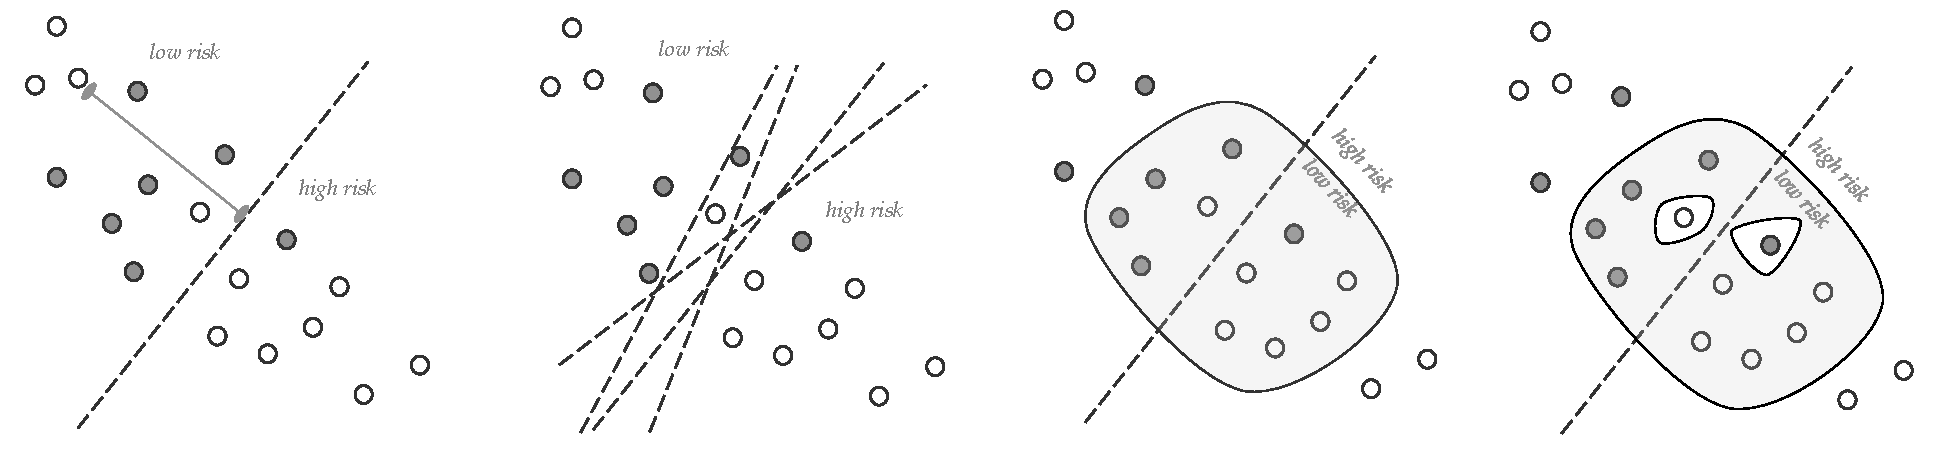
\includegraphics[width=\textwidth]{figures/active_learning.pdf}

\caption{A comparison of different query selection strategies for active learning on a non-stationary distribution. The shaded and empty circles are training data from two classes, $0$ and $1$ respectively. The red empty circles are samples from a new distribution (produced by executing the learned policy), and belong to class $1$. Typical strategies assign high risk to states close the decision boundary (a), or for which a set of estimators disagree (b). Neither of these apply to our new samples in red. In contrast, we use a strategy that is amenable to non-stationary distributions by assigning high risk to novel states (c) and states in historically mislabeled regions. 
%Confidence and Query by Committee methods measure
%{\color{blue} FP:estimate} states far away from the decision boundary of the estimator as having low risk,
%however novelty detection methods measure {\color{blue} FP:estimate} the level of risk as
%{\color{blue}FP:by} how far a point is from the trained data. Our
%modified risk method attempts to measure risk both as a function of how far it
%{\color{blue}it gramatically refers to risk,
%but you mean sample "it$\mapsto$a sample"?} is from data trained on
%{\color{blue}grammatically strange$\mapsto$from the training data} and the decision boundary of the estimator. 
}
\label{fig:support_example}
\end{figure*}

\emph{On-line}\adnote{inconsistency here beetween offline and on-line instead of online} imitation learning approaches such as DAgger iteratively gather more examples from the supervisor \cite{grollman2007dogged,ross2010efficient,ross2010reduction}. In DAgger, a series of policies are learned.  In each iteration, the latest policy is "rolled out" (executed) and the supervisor provides demonstrations for the  new stats, which are then aggregated with the previous examples for the next iteration. The number of mistakes in DAgger scales linearly with the time horizon \cite{ross2010efficient}. DAgger and related algorithms have been applied in a wide range of applications, from quadrotor flight to natural language to Atari games~\cite{NIPS2014_5421,duvallet2013imitation,ross2013learning}.

One drawback is that such online algorithms increase the burden on the supervisor. Our goal is to reduce supervisor burden without degrading robot performance, \emph{by only requesting demonstrations for risky states. }

Risk arises because:  (1) states are different than the states previously encountered and used to generate the current policy, i.e., they can be considered novel or outliers \cite{hodge2004survey}; or (2) states are in a region that  has been historically misclassified. 
%\adnote{Ken's version below does not seem to represent what we actually do.}
%the action associated with a state under the current policy yield a resulting state that is inconsistent with the expected next state. [how do we measure 2? - Ken]

We introduce the SHIV algorithm (Svm-based reduction in Human InterVention), which reduces supervisor burden by enabling the robot to only request supervision for risky states. SHIV uses stream-based active learning with a query selection method that evaluates risk in a manner tailored to non-stationary state distributions (like those encountered when executing a new policy at each iteration). It builds on the One Class SVM method for approximating quantile level sets \cite{scholkopf2001estimating}.




We compare SHIV with DAgger in three experiments: 1) a driving simulator, 2) 6DOF robot arm push-grasping in clutter (simulation with Box2D), and 3) surgical needle insertion. Our analysis suggests that compared to DAgger, SHIV learns a policy that performs significantly better given the same amount of human supervision. Conversely, SHIV significantly reduces supervisory burden (by a factor of \adnote{fill in}) while achieving the same performance. 







% \adnote{Old intro:}

% Consider the problem of teaching a robot a complex task such cooking a meal or as racing a toy car around a track
% against human opponents. When the robot is only provided with visual demonstrations without the knowledge or an
% underlying cost function describing the task, traditional model based control approaches are often not applicable. In
% these situations, the learning from demonstrations (LfD) approach provides a paradigmn for teaching a robot how to
% accomplish the task \cite{ross2013learning,pomerleau1989alvinn,schulman2013case}.\adnote{these are very random things to cite for LfD, FYI - there is a survey by Argall that usually gets cited}

% One approach to LfD is to train a policy, or a function estimator (either a classifier or regressor), to predict a
% supervisor's behavior given training data consisting of pairs of observations (input) and actions (output) performed
% while accomplishing a task. Since the robot's actions typically affect the resulting next state, the resulting sequences
% of states encountered during the execution of a policy are not independent random variables, thus making statistical
% inference challenging. Ross et al. proved that this can cause the error in the policy estimator to compound over the
% time and lead to performance degradation that is proportional to the time horizon of the task squared. The intuition
% behind this result is that as the robot makes mistakes with respect to the supervisor's policy it drifts from the
% distribution it was trained on and might encounter new states it can't generalize to.  Ross and Bagnell overcome this by
% presenting an iterative method that first trains a policy on the data observed using standard supervised learning
% techniques then tries (or 'rolls out') the policy out in the environment to see what states are likely to occur under
% the robot's trained policy.  The supervisor then tells the robot what controls it should applied after each iteration
% and the policy is retrained \cite{ross2010reduction}. The DAgger method has been successfully used since to teach a
% robot how to follow verbal instructions, achieve state of the art performance on Atari games and fly a quad copter
% through a forest~\cite{NIPS2014_5421,duvallet2013imitation,ross2013learning}.






% During learning, implementations of DAgger require the supervisor to manually provide control inputs that the robot
% should have applied for each states it visits when rolling out the current best policy estimate. If the supervisor is a
% human or an algorithm with a high time complexity, this can be tedious and expensive. We are hence interested in
% reducing the burdon on the supervisor by partitioning the state space into states where the policy can either be
% executed autonomously with little expected risk, or where supervisor control input (or 'labels') are likely to be
% required due to high 'risk'. A state can be risky for 2 reasons: 1) we encounter a state which has a low density of
% training data in its vicinity, which potentially means our policy will mis-predict the supervisor
% \cite{tokdar2010importance} 2) the state is near previously visited states, but the control-input is mis-predicted
% nonetheless. If an accurate density estimation corresponding to
% the pairs of visited states and control signals is available, the first scenario can be captured by regions of
% state-space with a low density estimate. Areas of low density are then considered to be risky since an insufficient data
% is available to accurately model the demonstrator's policy. This idea is also captured in the notion that 'a trained
% model will be able to generalize within the distribution it is trained on' \cite{tokdar2010importance} in statistical
% machine learning. The second case arises for example when the current best policy estimate is locally inconsistent with supervisor
% demonstrations.
% %
% %Vague!!!
% %This property can be seen used in importance sampling when data is collected from one distribution, but tested on
% %another and has to be re-weighted %to the test distribution \cite{huang2006correcting}. 
% %
% While the amount of data needed to accurately estimate the density increases exponentially with the dimension of state
% space \cite{nadaraya1964estimating}, we can turn to approximate methods which instead attempt to learn an approximate
% representation of the quantile levelsets of the distribution. Thus, we propose using a modified version the One Class
% SVM method for support estimation that only tries to estimate the level set of the quantile function of the density
% \cite{scholkopf2001estimating} at a user-determined quantile threshold which has been used even with high-dimensional
% image data \cite{liu2014unsupervised}. Our modification furthermore removes areas of state space from the super-levelset
% estimate where the local policy estimate is inconsistent with the supervisor demonstrations.

% To apply our approach, we make the same assumptions as in the case of DAgger: 1) we require access to an environment
% where a robot can try out (roll out) policies to sample trajectories and where we are able to collect observation states
% and corresponding control inputs along these trajectories. 2) an interface allowing a supervisor to provide control
% inputs that should have been applied for states along parts of the rolled out trajectories. 3) We assume that we are
% able to collect a series of observations from the environment and the controls applied. 4) Lastly, for our theoretical
% analysis to apply, we assume the current observation only depends on the previous observation and control input (i.e.
% the Markovian assumption).

% Our core contribution is the extension of DAgger to \acro~which incorporates a notion of risk to learning from
% demonstrations and reduces supervisor
% burdon by asking for supervisor demonstrations only in `risky' states. 
% We achieve this by proposing a modified version of the One Class SVM, that both estimates the quantile level sets 
% of the distribution of states with demonstrations and additionally
% and carves out areas in the support where we know our policy will mis-predict the supervisor, thus identifying states of high
% risk.  Our experimental results on a Super Mario Atari video game,  suggest \acro~is able to reach DAgger's
% peak performance of surviving for an average of 2200 simulation steps with only 1200 queries to the supervisor, while DAgger required 2800 queries
% averaged over 20 levels.
% {\color{blue}[-- FINALIZE --]}


\section{Related Work}
Below we summarize related work in active approaches to robot learning from demonstration, as well as in risk evaluation techniques that we build upon. 

\noindent\textbf{Active Imitation Learning.}
SHIV instantiates \emph{stream-based} active learning ~\cite{atlas1990training,cohn1994improving}. It iteratively receives the stream of states induced by executing the current best policy estimate, and actively decides for each state whether to query the supervisor or not.

Stream-based active learning has two ingredients: a stream, given here by executing the current best policy, and a query selection method deciding whether or not to query. Typical query selection methods are estimator-centric: they evaluate the estimator's confidence, e.g. distance from the classification hyperplane \cite{tong2002support}, as in Fig. \ref{fig:support_example}(a). An alternative to distance-based measures of confidence is query by committee \adnote{cite}, which uses a committee of hypothesized estimators that are trained on different subsets of the training data. Confidence here is based on the level of agreement or disagreement among these hypotheses, with higher levels of disagreement for a state leading to higher chances of querying that state (Fig. \ref{fig:support_example}(b)).

Both approaches implicitly assume a stationary state distribution --- that the new data is sampled from the same distribution as the previous training data. Although such methods have been previously proposed for online imitation learning (see \cite{chernova2009interactive,grollman2007dogged} for the former and \cite{judah2011active,judah2012active} for the latter),
online imitation learning violates the stationary distribution assumption because each new policy induces a new distribution of states. This can have negative consequences for learning: it has been shown that when training and test distributions are different, query by committee can perform worse than randomly selecting  which states to query \cite{burbidge2007active}.\adnote{merged the two types since they have the same problem, and references the figure}


In SHIV, we use a query selection method that allows for a non-stationary distribution, evaluating confidence based on \emph{novelty} (is the state an outlier to the training distribution), as in Fig. \ref{fig:support_example}(c). Additionally, we also assign lower confidence to  historically \emph{mislabeled} regions, as in Fig. \ref{fig:support_example}(d). %Our approach builds on the One Class SVM method for approximating quantile level sets \cite{}, which has already been used in novelty detection on high-dimensional image data \cite{}. 
Our results in Sec. \ref{}\adnote{fill in} suggest that this method is a better predictor of misclassification risk than a typical, estimator-centric query selector (be it distance or query by committee based).


\noindent\textbf{Risk via Novelty Detection.}
One part of our risk definition is the notion that a trained model will be able to generalize within the distribution it is
trained on \cite{tokdar2010importance}. Novelty detection \cite{hodge2004survey} is concerned with recognizing that a sample is outside of this distribution, making it difficult for a model to correctly predict its label.
One approach to novelty detection is to directly estimate the underlying probability density function from which the data is sampled. However, the amount of data needed to accurately do so scales exponentially in the number of dimensions \cite{nadaraya1964estimating}.

An alternative to evaluating the probability of a data point is to measure distance to its nearest neighbors \cite{knox1998algorithms}. However, this approach was shown to be
susceptible to outliers since nearest neighbors mostly incorporate local information about the data \cite{hodge2004survey}.

Our approach is based on the One Class SVM proposed by Scholk{\"o}pf et al., which estimates a particular quantile level set for the training data by solving a convex quadratic program  to find support
vectors. The method has been theoretically shown to approximate the quantile levelset of a density estimate
asymptotically for correctly chosen bandwidth settings and in the case of a normalized Gaussian kernel function \cite{vert2006consistency}. 
In \cite{liu2014unsupervised}, the One Class SVM has furthermore been used for novelty detection in high-dimensional 
image data.

% The field of learning from demonstrations has achieved state of the art performance in a variety of areas within robotics
% \cite{argall2009survey}. Abbeel et al.~used an iLQR controller based on helicopter trajectories demonstrated by a human supervisor
% to successfully learn a series of aerobatics stunts \cite{abbeel2007application}. Billard and Matari used a hierarchy of
% neural networks on video data and tracking markers to imitate the movement of human arms on a 37 degree of freedom humaniod
% robot \cite{billard2001learning}. Schulman et al. used a non-linear warping technique based on thin-plate splines
% to transer demonstrations of a human controlling a PR2 robot to tie knots with a rope to new and unseen initial
% configurations of the~\cite{schulman2013case}. 

% A subset of research in the field of learning from demonstrations is working within the assumptions that the dynamics of
% the robot and the environment are not known and that no access to a cost function describing a given task is available.
% Under these assumptions, a set of trajectories and controls can be collected from a supervisor and the policy learning
% problem can be treated as a supervised learning problem that determines a function from state space to
% controls~\cite{argall2009survey} by means of regression. Pomerleau et al. used this approach on raw image data and
% associated control inputs provided by a person driving a car. The authors then learned a policy that allowed a car to
% travel on a highway. However, they observed that if the car deviated from the middle of the road the learned policy was
% not able to recover, this behavior was attributed to the fact the car only drove in middle of the road while collecting
% demonstrations~\cite{pomerleau1989alvinn}. Ross et al. studied this effect and showed that error can accumulate at a
% rate quadratic in the time horizon of the policy in general. Ross et al. then proposed a learning algorithm, SMILE, that
% stochastically mixes the supervisor's control with the robot's policy control signal during training, thus allowing the
% robot to explore states the supervisor had not visited during training~\cite{ross2010efficient}. 

% Ross and Bagnell improved upon this method with DAgger (Dataset Aggregation) -- an iterative method that first trains a
% policy on the data observed using standard supervised learning techniques and then tries, or 'rolls out' the policy in
% the environment to see what states are likely to occur under the policy. The supervisor then tells the robot what
% controls it should applied at each stage of this roll-out and the policy is retrained with an aggregate of all data seen
% before \cite{ross2010reduction}. This algorithm has found widespread adoption in the robotics community. in
% \cite{ross2013learning}, a quad-copter using DAgger learned how to fly through a forest using only Histogram of Gradient
% (HOG) features extracted from camera images \cite{ross2013learning}. Guo et al. combined DAgger with Deep Q-learning
% methods to achieve state of the art performance on a common Atari game benchmark in Reinforcement Learning
% \cite{NIPS2014_5421}. Duvallet et al. furthermore used DAgger to teach robots to follow verbal instructions about where
% to move sematically in a building with a training set consisting of of humans following similar verbal instructions
% \cite{duvallet2013imitation}. Levine et al. very recently extended the iterative learning paradigm through Guided Policy
% Search, which replaces the supervisor with iLQG and uses KL-divergence constraints to train the policy~\cite{levine2015end}.  


% One limitation of DAgger which we address in the present work is that it requires the demonstrator, or supervisor, to
% provide control inputs that the supervisor would have applied for every state encountered along a roll-out of a trajectory at every interation of the
% algorithm. Providing these control inputs can be very tedious or expensive both in the case where the `supervisor' is a
% human or an algorithm with a high computational demand.

% In prior work, Judah et al. proposed applying active learning techniques to improve the learninng ability of an algorithm given a fixed budget. 
% \cite{judah2011active,judah2012active}. A drawback of this approach is that it requires us to estimate a complete
% density of states from the samples, which can be difficult especially in high dimensions. Furthermore, the  
% at each iteration only one labeled state was given. Thus, the robot could potentially be required to try out many more iterations of learning in order to successfully accomplished the task.  

% \begin{enumerate}
% \item Our work is different than traditional pool base active learning for two reasons 1) the data comes in as a stream (i.e. we decided whether to label or not label the sample vs. using a pool base methods) 2) the estimator being trained is part of the parametrization of the distribution of states being encountered at run time, thus violating the i.i.d assumption common in these methods. 
% \item Some techniques that can handle these approaches are 1) uncertainty sampling , or measuring some confidence level in a classifier and deciding whether to label or not. 2) Query by committee, which involves sampling a committee of hypothesises from a version space of consistent classifiers 3) Density weighted model, which fitting a density to the unlabeled pool and then using a technique such as uncertainty sampling or query by committee to chose the label with the highest uncertainity times the density under the model. The reason for density weighted model is because the previous approaches are prone to labeling outliers \cite{settles2008analysis}. 
% \item Our approach can be considered a query selective strategy that uses the ideas of density weighted models. The level set estimation of the One Class SVM is a binary decision metric of how close a point is to the global support points that define its neighbors. Then our hole punching technique places a "prior" on points that are likely to be misclassified condition on the fact that points nearby are misclassified. Thus, encapsulating both a notion of uncertainity and distance to relative points. 
% \item One point that I've been thinking about is that traditional active learning is about training an estimator on some fix distribution and then trying to predict how the estimator will change given new points sampled from the same distribution. Thus most approaches work on the estimator themselves (query by committee sampling different hypotheses or uncertainty sampling measuring confidence). This assumption is violated in DAgger because you are sampling from a new distribution each iteration different from what is trained on. Thus, a confidence threshold such as (distance to hyperplane for an svm) would be misleading because if the point was drawn from a different distribution it could be very far from the hyperplane, but have a different label than that side of the hyperplane. Thus, we purpose not looking at the estimator but at the data itself. We make an assumption that points close to other points in our feature space will have similar labels, but the outliers are unknown and will need new labels. I suggest we run a uncertainty sampling technique vs. SHIV to verify all this. 

% \end{enumerate}



% %[Let's discuss this part]
% {\color{blue}[-- IMPROVE THIS PARAGRAPH --]} In order to determine state space regions where a policy is likely to determine
% an incorrect control input, we leverage a
% property in statistical machine learning that a trained model will be able to generalize within the distribution it is
% trained on \cite{tokdar2010importance}. This property is used in importance sampling when data is collected from one
% distribution, but tested on another and has to be re-weighted to the test distribution \cite{huang2006correcting}. One
% approach is to estimate the probability density of states the policy is trained on. However, the amount of data needed to accurately estimate the density scales exponentially in the number of \cite{nadaraya1964estimating}.

% Several alternative approaches have been proposed to determine regions of state-space where an estimator is likely fail
% to generalize away from the training-data \cite{markou2003novelty}. Knox and Ng \cite{knox1998algorithms} used a nearest
% neighbor-based approach by estimating if a point was close to $k$ neighbors, however this approach was shown to be
% susceptible to outliers since nearest neighbors mostly incorporate local information about the data. Manevitz and Yousef
% \cite{manevitz2002one} trained a neural network filter to try and reconstruct the data and when the reconstruction error
% at a point was high, the point was considered as likely to be outside of the estimators domain within which
% generalization was possible. Manevitz and Yousef conjecture  that finding the right architecture can be task specific
% and might require a large amount of hyperparameter tuning.

% Our approach is in particular based on the One Class SVM proposed by Scholk{\"o}pf et al. which estimates a user
% defined quantile level set for a collection of training data by solving a convex quadratic program  to find support
% vectors. The method has been theoretically shown to approximate the quantile levelset of a density estimate
% asymptotically for correctly chosen bandwidth settings and in the case of a normalized Gaussian kernel function \cite{vert2006consistency}. 
% In \cite{liu2014unsupervised}, the One Class SVM has furthermore been used for outlier detection of high-dimensional 
% image data.






\section{Problem Statement}
\noindent\textbf{Policies and State Densities.}
We denote by $\mathcal{X}$ the set consisting of \emph{observable states} for a robot task, consisting, for example, of
high-dimensional vectors corresponding to images from a camera, or robot joint angles and object poses in the environment.
We furthermore consider a set $\mathcal{U}$ of \emph{allowable control inputs} for the robot, which can be discrete or
continuous. We assume Markovian dynamics, such that the probability of state $\mathbf{x_{t+1}}\in
\mathcal{X}$ can be determined from the previous state $\mathbf{x}_t\in\mathcal{X}$ and control input $\mathbf{u}_t\in
\mathcal{U}$. Thus, we assume that 
$$p(\bx_{t+1}|\bu_{t},\bx_{t}, \ldots, \bu_{0}, \bx_{0})=p(\bx_{t+1}|\bu_{t}, \bx_t)$$
We assume a probability density over initial states $p(\bx_0)$.
%We denote the probability density over the initial state also by $p:\mathcal{X}\to \mathbb{R}$. 

A trajectory $\hat{\tau}$ is a finite series of $T+1$ pairs of states visited and corresponding
control inputs at these states, $\hat{\tau} = (\mathbf{x}_0,\mathbf{u}_0, ...., \mathbf{x}_T,\mathbf{u}_T)$, where $\bx_t\in \mathcal{X}$
and $\bu_t\in \mathcal{U}$ for $t\in \{0, \ldots, T\}$ and some $T\in \mathbb{N}$.  
For a given trajectory $\hat{\tau}$ as above, we denote by ${\tau}$ the corresponding trajectory in state space,
${\tau} = (\bx_0,....,\bx_T)$.


A policy is a function $\pi: \mathcal{X} \to \mathcal{U}$ from states to control inputs. 
We consider a space of policies $\pi_{\theta}:\mathcal{X}\to \mathcal{U}$ parameterized by some $\theta\in \mathbb{R}^d$. Any such policy $\pi_{\theta}$ in an environment with probabilistic initial state density and Markovian dynamics
induces a density on state-space trajectories of length $T+1$: $$p(\tau | \theta)=
p(\bx_0)\prod_{i=0}^{T-1}p(\bx_{t+1}|\pi_{\theta}(\bx_t),\bx_t)$$


Let $p(\bx_t|\theta)$ denote the value of the density of states visited at time $t$ if the robot follows the policy
$\pi_{\theta}$ from time $0$ to time $t-1$.\adnote{shouldnt you then define this above insted of the probability of a trajectory?} This density can be computed by marginalization: $p(\bx_t|\theta) =
\int_{\bx_{t-1}}...\int_{\bx_1} p((\bx_t,...,\bx_1)|\theta) d\bx_{t-1}...d\bx_1$. Following \cite{ross2010reduction}, we can compute
the average density on states for \emph{any} timepoint by 
\begin{equation}
p(\bx|\theta) = \frac{1}{T} \sum^T_{t=1} p(\bx_t|\theta)
\label{eq:density}
\end{equation}


While we do not assume analytic knowledge of the distributions corresponding to: $p(\bx_{t+1}|\bx_t,\bu_t)$, $p(\bx_0)$, $p(\bx_{\bx}|
\bx)$\adnote{this is a typo} or $p(\bx|\theta)$, we assume that we have a stochastic real robot or a simulator such that for any state
$\bx_t$ and control $\bu_t$, we can sample the $\bx_{t+1}$ from the density $p(\bx_{t+1}|\pi_{\theta}(\bx_t),\bx_t)$. 
Therefore, when 'rolling out' trajectories under a policy
$\pi_{\theta}$, we utilize the robot or a simulator to sample the resulting stochastic trajectories rather than
estimating $p(\bx|\theta)$ itself.

\noindent\textbf{Objective.} Typically, the objective of policy learning is to find a policy that minimizes some known cost function
$C(\tau) = \sum^T_{t=1} c(\bx_t,\bu_t)$ of a trajectory $\tau$. The cost function $c:\mathcal{X}\times \mathcal{U}\to \mathbb{R}$ is typically user defined and task specific. 
For example, in task of inserting a peg into a hole, the distance between the peg's current and desired final state can
be considered \cite{levine2015end}.  
In our learning from demonstration setup, the robot does not have access to the cost function itself. Instead, it only has access to 
a `supervisor' that we assume uses some near-optimal policy $\tilde{\pi}$ to minimize $C(\tau)$. We are furthermore given
an initial set of $N$ stochastic demonstration trajectories $\lbrace \tilde{\tau}^1,...,\tilde{\tau}^N \rbrace$. 
which are the result of the supervisor applying this policy. This induces a training dataset $\mathcal{D}$ of all state-control input pairs from the demonstrated trajectories. The goal is to produce a low cost policy for the task based on these demonstrations.

We define a `surrogate' loss function $l:\mathcal{U}\times \mathcal{U}\to \mathbb{R}$, which provides a distance
measure between any pair of control values. In the continuous case, we consider $l(\bu_0,\bu_1) = ||\bu_0-\bu_1||^2$,
while in the discrete case $l(\bu_0,\bu_1) = 1$ if $\bu_0 \neq \bu_1$ and $l(\bu_0, \bu_1)=0$ otherwise.

Given a candidate policy $\pi_{\theta}$, we then use the surrogate loss function to approximately measure how "close" the policy's
returned control input $\pi_{\theta}(\bx)\in \mathcal{U}$ at a given state $\bx\in \mathcal{X}$ is to the supervisor's policy's control output
$\tilde{\pi}(\bx)\in \mathcal{U}$. 

Following \cite{ross2010reduction}, our objective then consists of determining a policy $\pi_{\theta}$ minimizing the expected surrogate loss, where the expectation is taken over the distribution of states induced by the policy across any time point in the horizon:

 \vspace{-2ex}
\begin{align}\label{eq:LFD_obj}
\underset{\theta}{\min} \: E_{p(\bx|\theta)} [l(\pi_\theta(\bx),\tilde{\pi}(\bx))].
\end{align}
with $p(\bx|\theta)$ from Eq. \ref{eq:density}.

If the robot could learn the policy perfectly, this state density would match the one encountered in the user examples. But any small error will make the state distribution deviate from the training one, and this the motivation for an iterative algorithm like DAgger and now SHIV.

% The optimization problem in Eq. \ref{eq:LFD_obj} is  typically non-convex. It can also be difficult to solve, since we only have access to samples from the supervisor's policy $\tilde{\pi}$ arising from the demonstration trajectories $\mathcal{D}$. To address these issues Stephane and Ross proposed an iterative method known as DAgger \cite{ross2010reduction}.

\section{SHIV}
\adnote{putting shiv and dagger side by side. also, notice how I am setting up the rest of the section by explaining what will follow; also, avoid filler sentences like "note that ..." when you are not following that up with a point; avoid filler words like two "basic" steps -- it's just steps, why are they basic?}

Both SHIV and DAgger \cite{ross2010reduction} solve the minimization in Eq. \ref{eq:LFD_obj} by iterating two steps: 1) find an optimal $\theta$ using the training data $\mathcal{D}$ thus far, and 2) execute the policy induced by the current $\theta$, and ask for labels for the encountered states. However, instead of querying the supervisor for every new state, SHIV will actively decide whether the state is risky enough to warrant a query, thereby reducing supervisory burden.

%  \subsection{DAgger: Dataset Aggregation}
% Note that Eq. \ref{eq:LFD_obj} involves both the parameterized policy $\pi_{\theta}$ and the average distribution of
% states with respect to the policy, $p(\bx|\theta)$. Let us recall that Dataset Aggregation (DAgger) is an iterative algorithm developed by \cite{ross2010reduction} which iterates two basic steps for $K$ iterations to find an optimal policy under this objective. 
%DAgger iteratively minimizes $\pi_{\theta}$ on the collected dataset of examples $\mathcal{D}$ and then adds new states
%of high probability under $\pi_\theta$ by sampling via policy `roll outs' from $p(\bx|\theta)$. 
%\fpnote{DAgger and \acro~formal algorithms side by side would be better, also the Step 1/2 below can be
%made more precise then and refer to the algorithm}

\subsection{Step 1.}
The first step of any iteration $k$ is to find a $\theta_k$ that minimizes surrogate loss on the current dataset $\mathcal{D_k}=\{(x_i,u_i)|i\in\{1,\ldots,M\}\}$ of demonstrated state-control pairs (initially just the set $D$ from above):
% \fpnote{this is really start of iteration `i', as we circle back}
% At iteration $k=0$ an initial dataset $\mathcal{D}_0$ of $N_0$ supervisor demonstration trajectories 
% with $T+1$ time steps: $\tau^i=(\bx_0^i, \bu_0^i, \ldots, \bx_T^i, \bu_T^i)\in (\mathcal{X}\times\mathcal{U})^{T+1}$ for $i\in \{0, \ldots, N_0\}$
% mapping states to control
% inputs is provided. DAgger solves the following optimization problem with respect to the surrogate loss function:

 \vspace{-2ex}
\begin{align}\label{eq:super_objj}
\theta_{k} = \underset{\theta}{\argmin} \: \sum_{i=1}^{M} l(\pi_{\theta}(\bx_i),\bu_i).
\end{align}

\adnote{simplified D above to just be pairs so that shiv makes sense too, as it doesnt add full trajectories}
This problem can be treated as a supervised learning problem which can be solved using standard machine
learning techniques, for example a support vector machine or a neural network. 
 
To handle the fact that the supervisor's policy can be noisy, a zero-mean noise term $\epsilon$ 
can be considered as present in policy's output. We employ a regularization technique in the optimization which is
used to control the smoothness of the function that is fit to the sampled data. In practice this regularization corresponds to a penalty term on either the L2 norm on the weights for regression based techniques or the slack coefficient for support vector machines \cite{scholkopf2002learning}.\adnote{is this just us or also dagger?}
 
 \subsection{Step 2}
The second step starts in both SHIV and DAgger by rolling out the policy $\pi_{\theta_{k}}$ to sample states that are likely to occur under $\theta_{k}$. 

What happens next, however, differs. For every state visited, DAgger requests the supervisor to provide the appropriate control/label. Formally, for a given sampled trajectory  $\hat{\tau} = (\bx_0,\bu_0,...,\bx_T,\bu_T )$, the supervisor provides labels $\tilde{\bu}_t$, where $\tilde{\bu}_t \sim \pi(\bx_t) + \epsilon$ for $t\in \{0, \ldots, T\}$.
The states and labeled controls are then aggregated into the next data set of demonstrations $\mathcal{D}_{k+1}$:
$$D_{k+1}=\mathcal{D}_k \cup \{(\bx_t,\tilde{\bu_t})\|t\in\{0,\ldots,T\}\} $$
%\fpnote{terms such as aggregated etc would be much clearer if we just refer to a particular line in the algorithm}

Providing correct control inputs or ``labeling'' at each
iteration and each state in DAgger can be tedious, imposing a large burden on the supervisor. \adnote{add in the discussion that another advantage of measuring risk is the early termination which can avoid disaster}
Instead of asking the supervisor for labels at all visited states $\{\bx_0,..,\bx_T\}$, SHIV uses a measure of \emph{risk} to actively \emph{decide} whether a label is necessary. For every state encountered $\bx_t$, it applies a \emph{decision function} $g_{\sigma}$, which we introduce in the next section, parametrized by a risk-sensitivity parameter $\sigma$ which will capture how smooth we expect the policy function to be: smoother functions imply that training examples have larger support, and data nearby will be less risky.

SHIV only asks for supervision on states for which $g(\bx)=-1$: \adnote{don't know what a good way to mention the termination condition is, maybe just a footnote or in discussion at the end as an advantage}
$$D_{k+1}=\mathcal{D}_k \cup \{(\bx_t,\tilde{\bu_t})\|t\in\{0,\ldots,T\},g(\bx_t)=-1\}$$

Steps 1 and 2 are repeated for $K$ iterations or until 
the cumulative surrogate is smaller than some predefined threshold\footnote{In the original DAgger the policy rolled out
was stochastically mixed with the supervisor, thus with probability $\beta$ it would either take the supervisor's action
or the robots. The use of this stochastically mix policy was for theoretical analysis. In practice, it is recommended
to set $\beta = 0$ to avoid biasing the sampling~\cite{NIPS2014_5421,ross2010reduction}}.


Dagger has been experimentally shown to perform well in both simulation and real world
    experiments\cite{}\adnote{cite}. Under a `no regret' assumption, Ross et al.\cite{ross2013learning} furthermore
deduced error bounds on the expected loss, which scale linearly in the time horizon $T$ --- as opposed to offline methods which scale quadratically. For a conservative $\sigma$, the SHIV performance is analogous to DAgger without asking the expert when it is absolutely not necessary. However, if $\sigma$ is too high, then SHIV will not collect new data that is needed and revert back to the performance of offline methods. We analyze the dependence on $\sigma$ in our experimental section. Our results suggest that SHIV is robust to this parameter selection. \adnote{must add this experiment!}

\subsection{Measuring Risk}

\adnote{somewhere in this section refer to the second figure}

% However, policy rollouts can in practice result in the robot entering dangerous states. For example, when DAgger was used on a
% quad-copter, the robot repeatedly crashed into trees before successfully learning to avoid them \cite{ross2013learning}.
We work under the assumption that a state can be risky for 2 reasons: 1) it lies in an area with a low density of
previously trained states, which can cause our policy to mis-predict the supervisor and incur high surrogate
loss \cite{tokdar2010importance}, or 2) the surrogate loss of the current policy at the current state is high, so that the state, although visited, does
not model the supervisor's control inputs correctly. 

% To address these limitations, we propose to 1) avoid highly risky states entirely by early termination of the policy
% roll-outs that enter these regions and 2) to recognize non-risky states and to not request supervisor input for these,
% thereby reducing the burden on the human trainer. 



%One way to do this is to define risk in terms of distance to a nearest neighbor, but this approach is vulnerable to
%outliers in the known set of states. Another option is to fit a density to the known set of states, which requires an
%exponential number of samples in the dimension of the state space \cite{nadaraya1964estimating}.\adnote{this stuff is in the related work too} 

To evaluate risk in high-dimensional state spaces (such as HOG features on images, like in our driving simulator testcase), we use
modified version of the technique known as the One Class SVM that implicitly approximately estimates a boundary of a user defined quantile of
a density representing the training data in $\mathcal{X}$ \cite{scholkopf2001estimating}.
%\fpnote{Refer to figure, replace "one way to do"  by "an approach to this problem is to" or similar - less informal}


%\subsection{Estimation of Quantile Level Sets}\label{sec:level}
\fpnote{my git commit on this section was overwritten by an old commit at version 10 - reintroduced modifications here,
Michael, please check this is still accurate with recent modifications}
We consider the problem of estimating the quantile level-sets of a distribution $P$ on a set $\mathcal{X}$ by means of a finite set of
independent and identically distributed samples $\mathbf{x}_1,...,\mathbf{x}_n\in \mathcal{X}$.
In most general terms, the quantile function for $P$ and subject to a class of measurable subsets $\mathcal{G}$ of $\mathcal{X}$ is
defined by
\begin{align}\label{eq:quantile}
U(\gamma) = \mbox{inf} \lbrace \lambda(G):P(G) \geq \gamma, G \in \mathcal{G} \rbrace \: 0<\gamma \leq 1
\end{align} 
$\lambda:\mathcal{G}\to \mathbb{R}$ above denotes a volume measure which most commonly is given by the Lebesgue measure.
Suppose furthermore that $G:[0,1]\to \mathcal{G}$ assigns a set $G(\gamma) \in \mathcal{G}$ that attains the infinum
measure (i.e. volume) for each $\gamma\in [0,1]$ (this set is in general not necessarily unique). 
$G(\gamma)$ denotes a set of minimum measure $G \in \mathcal{G}$ with $P(G(\gamma))\ge \gamma$. Note in particular that $G(1)$ is the support of the density $p$ corresponding to $P$, if $p$ exists. 

To handle distributions defined on high-dimensional spaces $\mathcal{X}$, work by Scholk{\"o}pf et al. looked at representing the class $\mathcal{G}$ via a kernel $k$ as the set of half-spaces in the support vector (SV) feature space \cite{scholkopf2001estimating}. 
By minimizing a support vector regularizer controlling the smoothness of the estimated level set function this work
derives an approximation of the quantile function described in Eq. \ref{eq:quantile}, which in particular has rigorous
convergence guarantees asymptotically when a normalized Gaussian kernel $k$ is chosen and bandwidths decay at an
appropriately chosen rate as the number of samples tends to infinity \cite{vert2006consistency}.
This approach can be thought of as employing $\lambda(G) = ||w||^2$, where $G_w = \lbrace x: f_w(x) \geq \rho \rbrace$,
$f_w(\mathbf{x}) = \sum_i w_i k(\mathbf{x}_i, \mathbf{x})$
and $(w,\rho)$ denote the weight vector and offset parameterizing a hyperplane in the feature space associated with a
Gaussian kernel $k(\bx_0,\bx_1) = e^{-||\bx_0 - \bx_1||^2/c}$.


Let $\Phi:\mathcal{X}\to \mathcal{F}$ denote the feature map corresponding to our exponential kernel, mapping the
observation space $\mathcal{X}$ into a Hilbert space $(\mathcal{F}, \langle, \rangle)$ such that $k(\bx, \bx') = \langle
\Phi(\bx), \Phi(\bx')\rangle$.

The One Class SVM proposed by \cite{scholkopf2001estimating} determines a hyperplane in feature space $\mathcal{F}$
maximally separating the input data from the origin:
\vspace{-2ex}
\begin{align}\label{eq:primal_sup}
    \underset{w\in \mathcal{F}, \mathbf{\xi} \in \mathbb{R}, \rho \in \mathbb{R}}{\mbox{min}}\: \frac{1}{2}||w||^2+\frac{1}{vn} \sum^n_i \xi_i - \rho\\
\mbox{s.t} \: \langle w,\Phi(x_i) \rangle \geq \rho - \xi_i, \: \xi_i \geq 0 \notag.
\end{align}

Here, the parameter $\nu$ controls the penalty or `slack term' and asymptotically approaches $\gamma$ \cite{vert2006consistency}
in the quantile definition when bandwidths decay at appropriate rates as the number of samples increases. The decision
function, determining point membership in the approximate quantile levelset is given by

\vspace{-2ex}
\begin{align}\label{eq:decision_func}
g_{\sigma}(x) = \mbox{sgn}(\langle w,\Phi(x) \rangle-\rho).
\end{align}
\adnote{let's make sure we define $\sigma$ above}

Here, for $x\in \mathcal{X}$, $g(x)=0$ if $x$ lies on the quantile levelset,
$g(x) = 1$ if $x$ is strictly in the interior of the quantile super-levelset and $g(x) = -1$ 
if $x$ lies strictly in the quantile sub-levelset. The dual form of the optimization yields a Quadratic Program 
that can be solved efficiently \cite{scholkopf2001estimating}. 

For training data in $\mathcal{X}$, we consider the quantile super-levelset for a user-defined threshold $\mu$ as a natural region within which
a trained policy $\pi_{\theta}$ can likely be learned since a sufficient data-density is available.
However, even when sufficient data is available, the associated control inputs may be inconsistent or noisy and a resulting policy
optimizing Eq. \ref{eq:super_objj} may still incur a large surrogate loss. To account for this, we propose a
modification to the One Class SVM:

\begin{align}
y_i = \left\{
     \begin{array}{lr}
         1 & : l(\pi_{\theta}(\bx_i),\bu_i)\le \varepsilon\\
         -1 & : l(\pi_{\theta}(\bx_i),\bu_i)>\varepsilon
     \end{array}
   \right.
\end{align}
Where, in the case when $l$ denotes discrete $0-1$ loss, we set $\varepsilon = 0$, while in the continuous $L_2$ loss
case, $\varepsilon$ is a user defined threshold specifying allowable surrogate loss.
We use $y_i$ to modify the One Class SVM optimization objective as follows: 

\vspace{-2ex}
\begin{align}\label{eq:primal_sup}
    \underset{w\in F, \mathbf{\xi} \in \mathbb{R}^l, \rho \in \mathbb{R}}{\mbox{min}}\: \frac{1}{2}||w||^2+\frac{1}{vn} \sum^n_i \xi_i - \rho\\
\mbox{s.t} \: y_i \langle w,\Phi(x_i)\rangle \geq \rho - \xi_i, \: \xi_i \geq 0 \label{eq:ineq}.
\end{align}

States that incur loss above the $\varepsilon$ threshold are then enforced to lie on the opposite side of the
hyper-plane separating the origin from the data in the feature space. Practically, this modification corresponds to
`carving out holes' in the estimated quantile super-levelset such that neighborhoods around states with $y_i=-1$ are
exluded from the super-levelset.

The dual formulation to the modified optimization problem, which is solved in practice, is 
\begin{align}\label{eq:dual_sup}
\underset{\alpha_i\in \mathbb{R}}{\mbox{min}} \sum_i^n \sum_j^n \alpha_i\alpha_j y_i y_jk(\bx_i,\bx_j)\\
\mbox{s.t} \: 0 \leq \alpha \leq \frac{1}{\nu n} \:, \sum_i^n \alpha_i = 1.
\end{align}

Our corresponding decision function $g_{\sigma}:\mathcal{X}\to \mathbb{R}$ is then derived in terms of the support vectors as $$g_{\sigma}(\bx) = \sum_i^n
\alpha_i y_i k(\bx_i,\bx) - \rho$$
To compute the $\rho$ term, we leverage the fact that for an optimal solution the
inequalities in Eq. \ref{eq:ineq} are equal for any $\alpha_j$ such that $0 < \alpha_j < \frac{1}{\nu n}$. Therefore we
can compute $\rho$ as  $\rho = \sum_i^n y_i \alpha_i k(\bx_i,\bx_j)$ \cite{scholkopf2001estimating} {\color{blue} [-- F:
explain this more --]}.

Our experiments analyze the performance of risk as a query selection strategy, with our without the addition of the second risk criteria --- regions of space where the surrogate loss is high.

% \subsection{The \acro~algorithm}

% Our proposed method trains a policy, $\pi_{\theta_k}$, but also estimates where the policy is likely to accurately
% predict the supervisor's control, by means of the thresholded surrogate just discussed.  
% % Too vague:
% %In the statistics community, a known property is that estimators are function will likely mis-classify if they are evaluated at points not in the distribution sampled from.
% %Techniques such as importance sampling use this results to train estimators on data drawn from a different distribution \cite{tokdar2010importance}.  
% To reduce the burden on the supervisor, we estimate the training data's quantile level-set for a user-defined threshold
% $\nu$ and further modify the corresponding super-levelset estimate by excluding neighborhoods of states that incur a loss
% above a threshold $\varepsilon$ chosen by the user.
% The user then only provides control input demonstrations for states of trajectory roll-outs that lie outside the
% resulting risk-aware quantile super-levelset.

% {\color{blue} [-- F: use formal algorithm and explain here instead --]} 
% \subsubsection{Step 1}

% Similar to DAgger, at iteration $k$, the algorithm estimates a policy, $\pi_{\theta_k}$ on the dataset $\mathcal{D}_k$
% by solving the optimization problem in Eq. \ref{eq:super_objj}. We then estimate the quantile super-levelset of the
% training data state-distribution solving the optimization for the modified One Class SVM using the dataset $\mathcal{D}_k$. 
% This yields a decision boundary $g_k(\bx)$, where is $g(\bx)\ge 0$ if a state $\bx$ is to be considered of `low risk' and $-1$ otherwise. 
 
 
%  \subsubsection{Step 2}
%  In DAgger, the policy $\pi_{\theta_k}$ is rolled out for a fixed number of time steps, however this could lead to the
%  robot entering pathological states that are risky. To prevent this, we terminate the rolled out policy if the risk, is
%  above some threshold $r(\bx_t) > r_0$.  Furthermore, instead of providing control inputs for every state, the supervisor is only required to 
%  provide demonstrations of control inputs for states for which $g(\bx)=-1$.  These demonstrations are then added to the
%  dataset $\mathcal{D}_{k+1}$ and the algorithm returns to Step 1. 

% We note that the choise of user-defined thresholds $\nu$, $\epsilon$, $r_0$ yield an implicit trade-off
% between exploration and exploitation. For large quantile super-levelsets, the robot is confident and asks the
% supervisor only rarely for demonstrations. Similarly, large $\varepsilon$ values allow the robot to be tolerant to
% incorrectly trained policies with large surrogate loss, while large $r_0$ settings allow the robot to explore risky
% areas and obtain more labels from the supervisor in those regions.


\section{Experiments}
All experiments were run on a machine with OS X with a 2.7 GHz Intel core i7 processor and 16 GB
1600 MHz memory in Python 2.7. The policies, $\pi_\theta$ were represented using either the linear SVM or  kernelized ridge regression classes in Scikit-Learn~\cite{scikit-learn}.

\subsection{Driving Example}
A common benchmark in Reinforcement Learning  is a car learning to drive around a track  \cite{argall2009survey}. To illustrate our methods ability in high dimensions, the car must follow a polygonal track using only HOG features extracted from images. If the car falls off the track, it is placed back on the center facing the angle of the polygonal track piece. We sample the polygonal track by drawing points from a Gaussian with a mean that is the centered of the video game work space. The convex hull of the sampled points is then computed. The car's control space $u = \lbrace -15^\circ, 0, 15^\circ \rbrace$ or 3 discrete commands that change the angle of the car. The internal state space of the car is xy-coordinates and the angle it is facing. Our supervisor is a solver that uses state space search through the driving simulator to plan the next control.

We have the supervisor drive around the track 2 times and then collect the raw images observed. We use a Gaussian Pyramids to down sample the images to $125 \times 125$ RGB pixels and then extract Histogram of Oriented Gradients (HOG) features using OpenCV,  where the size of $\bx$ is $27926$. For both DAgger and SHIV, we use a Linear Support Vector Machine (SVM) as the policy representation, with the regularization term on the slack variable $\gamma=0.01$, which was set via cross validation on the initial training examples from our supervisor. For the optimization of Eq. \ref{eq:dual_sup} in SHIV we used a radial basis function as well for the kernel with a bandwidth of $\lambda=0.01$ and $\nu = 0.95$ to account for $95\%$ of the training distribution. 

To compare our method against a traditional confidence based active learning approach, we use a confidence measure  of distance from the hyperplane \cite{tong2002support}. The threshold was set to the average distance from the hyperplane for the mis-classified points in $\mathcal{D}_0$, which consisted of two demonstrations from our solver. We further compared against Query By Committee, which was trained via bagging \cite{}. Our data set was uniformly divided up into 3 overlapping subsets each with $80\%$ of the data then for each subset a Linear SVM was trained on. If the three classifiers agreed with each other the point was determined low risk and if they disagree it was determined high risk. We finally compared our combined risk approach against the traditional One Class SVM without the "hole-punching". We measured the performance in terms of how many states are estimated to be of low risk (i.e. correctly classified) and are of actually high risk on the first policy roll out. Results  are averaged over 50 tracks and shown in Fig. \ref{fig:active_comp}. 


We compare performance in terms of minimization of the underlying cost function $c(\bx,\bu)$, which is the  number of times the car left the track versus the number of queries made to the supervisor. In Fig. \ref{fig:car_cost}, we plot the performance of DAgger and SHIV.  Initial results, which are run for 6 iterations each and are averaged over 40 levels, shown in Fig. \ref{fig:car_cost} suggest a $70\%$ reduction in the number of queries needed for SHIV compared to DAgger. 
 

\begin{figure}[t]
\centering
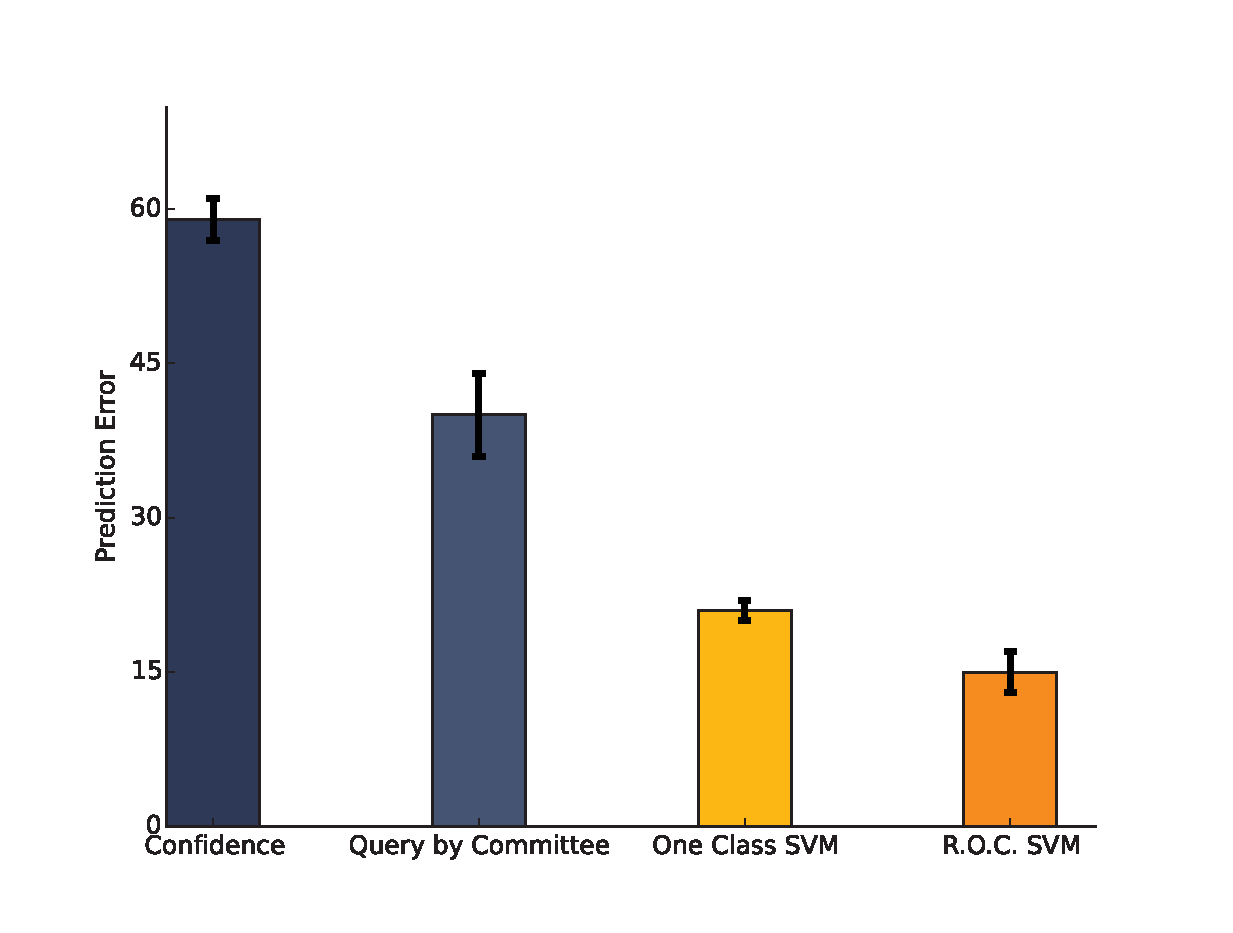
\includegraphics[width=9cm, height=8cm]{figures/risk_bar.eps}
   \caption { \footnotesize To compare our method against a traditional confidence based active learning approach, we use a confidence measure  of distance from the hyper plane \cite{tong2002support}. The threshold was set to the average distance from the hyper plane for the mis-classified points in $\mathcal{D}_0$, which consisted of two demonstrations from our solver. We further compared against Query By Committee, which was trained via bagging \cite{}. Our data set was uniformly divided up into 3 overlapping subsets each with $80\%$ of the data then for each subset a Linear SVM was trained on. If the three classifiers agreed with each other the point was determined low risk and if they disagree it was determined high risk. We finally compared our combined risk approach against the traditional One Class SVM without the "hole-punching". We measured the performance in terms of how many states are estimated to be of low risk (i.e. correctly classified) and are of actually high risk on the first policy roll out. Results  are averaged over 50 tracks.
   }

\label{fig:active_comp}
\end{figure}



\begin{figure}[t!]
\centering
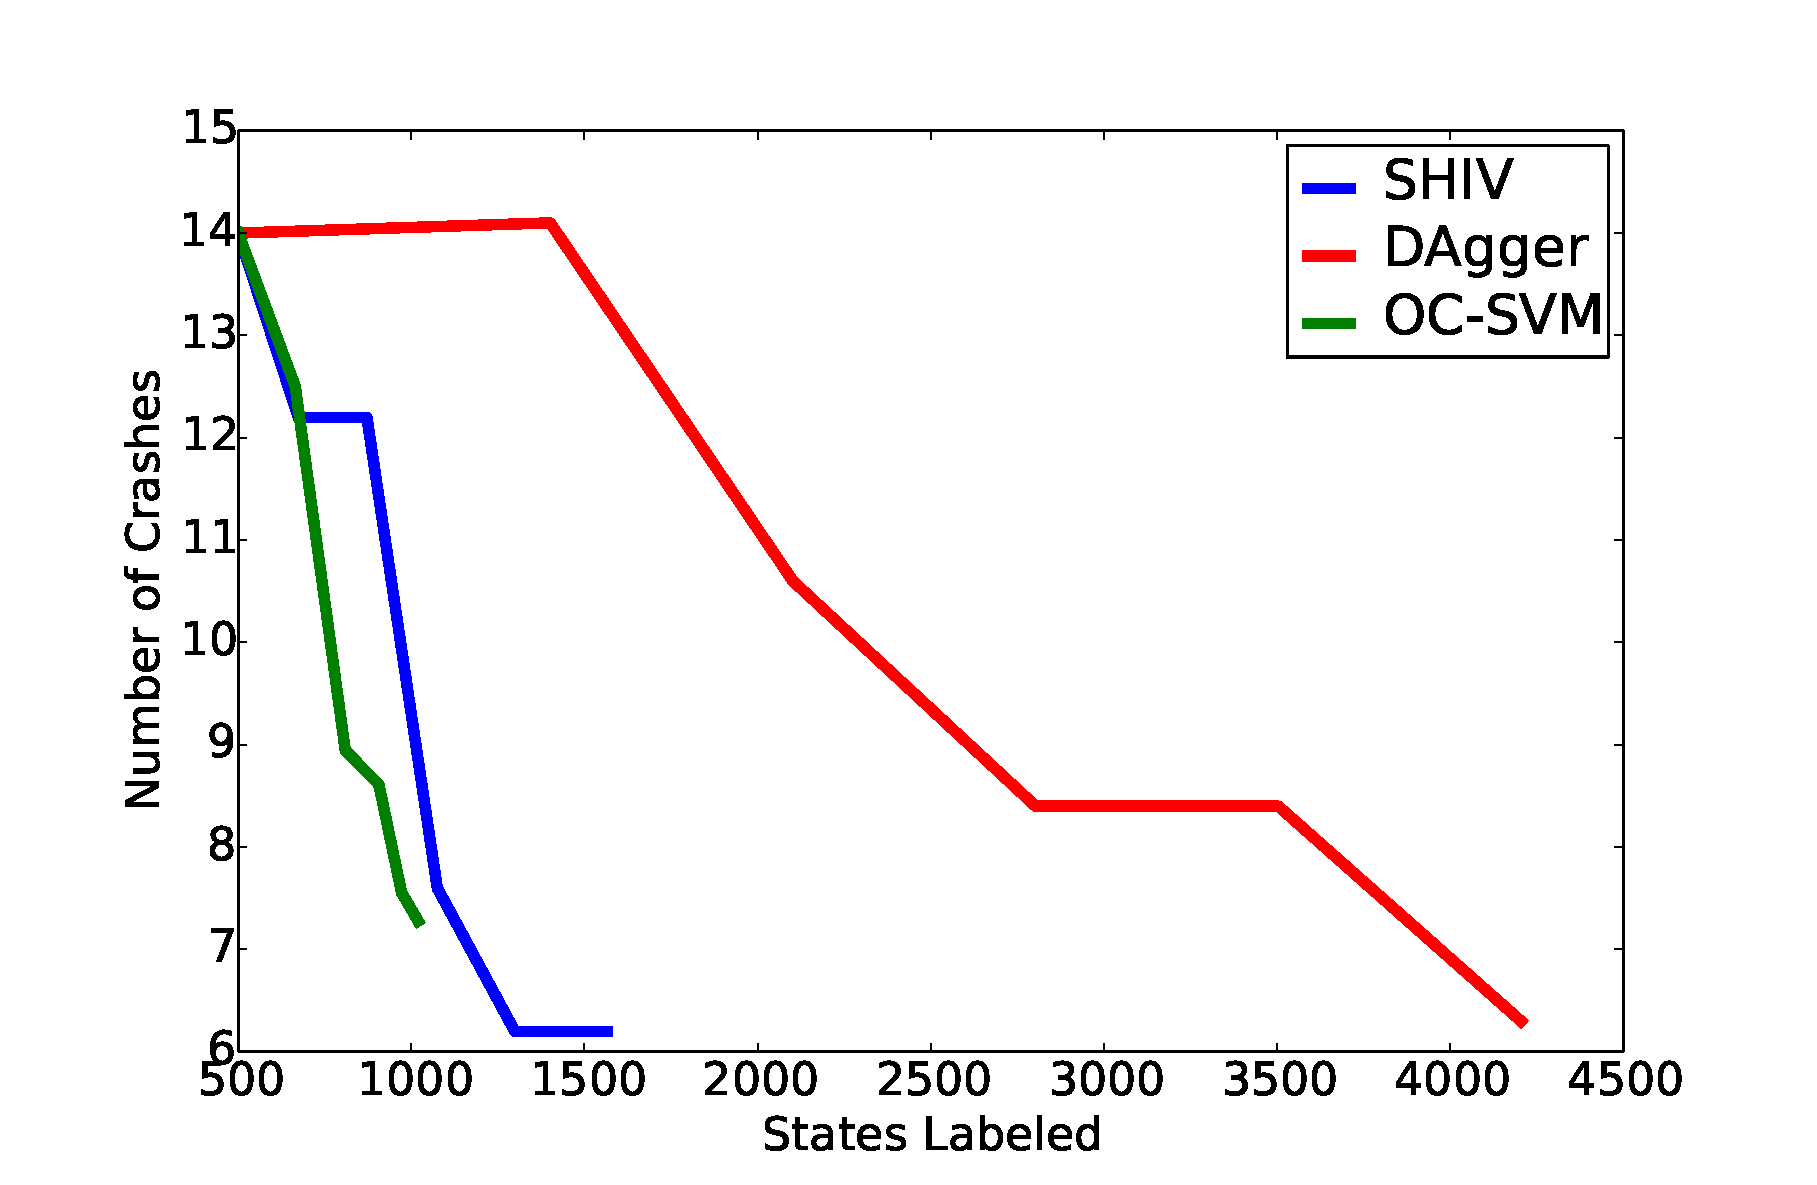
\includegraphics[width=8cm, height=6cm]{figures/dagger_shiv_one_class.eps}
\caption{We compare performance in terms of minimization of the underlying cost function $c(\bx,\bu)$, which is the  number of times the car left the track versus the number of queries made to the supervisor. In Fig. \ref{fig:car_cost}, we plot the performance of DAgger and SHIV.  Initial results, which are run for 6 iterations each and are averaged over 40 levels, shown in Fig. \ref{fig:car_cost} suggest an $70\%$ reduction in the number of queries needed for SHIV compared to DAgger,}
\vspace*{-10pt}
\label{fig:car_cost}
\end{figure}


\subsection{Grasping In Clutter}
To illustrate how our technique can be used in the continuous case and with a human demonstrator. 
We look at having a human demonstrator control a robot arm in 2D to reach a target object with out knocking other objects off a table. Grasping in clutter can be a challenging task because as shown in Kiteav et al. traditional motion planning techniques require knowledge of how the objects will behave when in contact. They used iLQR with a hand tuned cost function and dynamics given by a physics simulator to successfully grab an object without displacing the other movable objects on the table off \cite{kitaevphysics}. We are interested in learning such a policy via human demonstrations.   We used Box2D a physics simulator to model the virtual world. The arm, shown in Fig. \ref{fig:box2d_arm}, consists of 3 degrees of freedom and has a parallel jaw gripper. For input the human demonstrator provides controls through an XBox controller. The right joystick contains two principle components that determine the x and y velocity of the center of the end effector. The left bumper is a binary value for opening the gripper and the right bumper is a binary value for closing the gripper. Thus, the set of controls is the following tuple $\mathcal{U} = \lbrace [-1,1],[-1,1],\lbrace 0,1 \rbrace, \lbrace 0, 1\rbrace \rbrace$.  

Our state $\bx$ consisted of the 3 dimensional pose of the six objects on the table (translation and rotation), the 3 joint angles of the arm and a scalar value in the range $[0,1]$ that measured the position of the gripper, $1$ being fully closed and $0$ being opened. For our representation of $\pi_{\theta}$, we used kernelized ridge regression with the radial basis function as the kernel with the default Sci-Kit learn parameters. We defined the cost functions, $C(\bx,\bu)$, as the sum of the number of objects knocked off the table plus $10$ times the binary value indicating if the object is grasped or not. The order of magnitude difference in cost for grasping the object is to place emphasize on that portion of the task.  

In our experiment, we had our human demonstrator provide one demonstration and then iterated until the cost function was zero during the policy roll out. At each iteration, we sampled the pose of the target object from an isotropic Gaussian with a standard deviation that is equal to $3\%$ of the width of the table. 

In Fig. \ref{fig:grasp_cost} , we show the cost function $c(\bx,\bu)$ averaged over 8 trials for SHIV and DAgger. Initial results suggest we are able to achieve an approximate $70\%$ reduction in data. 

\begin{figure}[t!]
\centering
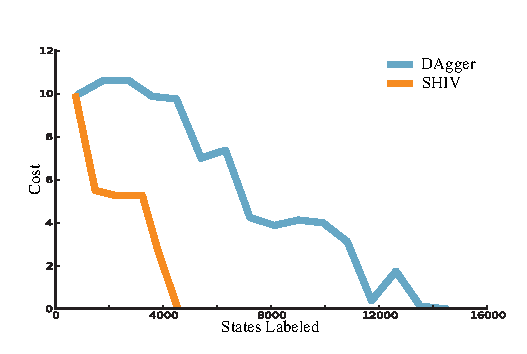
\includegraphics[width=\columnwidth, height=6cm]{figures/grasp_clutter.eps}
\caption{\todo{Might get more trials from Sammy tomorrow as well}We compare performance in terms of minimization of the underlying cost function $c(\bx,\bu)$, which is euclidean distance between translation in centimeters. In Fig. \ref{fig:car_cost}, we plot the performance of DAgger and SHIV without the modification.  Initial results, which are run for 20 iterations each and are averaged over 40 different initial starting positions, shown in Fig. \ref{fig:car_cost} suggest an $67\%$ reduction in the number of queries needed for SHIV compared to DAgger,}
\vspace*{-10pt}
\label{fig:grasp_cost}
\end{figure}




\subsection{Surgical Experiment}
Robotic Surgical Assistants (RSAs) are frequently used for procedures such as: prostectomy, uterectomy, and tumorectomies within the abdominal and thoracic cavities with high success rates~\cite{van2013laparoscopic,darzi2004impact} . Intuitive Surgical’s da Vinci Robotic Surgical Assistant, a type of RSA, facilitated over 570,000 procedures worldwide in 2014 across 3000 devices [5]. Currently, these devices are controlled by surgeons via physical tele-operation at all times; introducing autonomy of surgical sub-tasks has the potential to reduce cognitive load
and facilitate supervised autonomy for remote tele-surgerical procedures.

Suture tying in surgery is a manually intensive task that can occur frequently through out a surgery. One important step in suture tying is properly placing a needle in an initial configuration for insertion. Misplacement of this the needle can lead to suture failure and potentially rupture the surrounding tissue \cite{liu2015optimal}. In this experiment, we are interested in learning a policy to correct bad initial poses to the proper insertion pose as shown in Fig. \ref{fig:support_example}. We had a surgeon, Dr. Douglas Boyd, demonstrate via tele-operation the correction strategies. 

Dr. Boyd demonstrated a series of trajectories that started at an initial attempted needle insertion pose $P_0$ and applied the necessary corrections to achieve a goal pose $P_G$. We used three of these demonstrations as our initial dataset $\mathcal{D}_0$. Dr. Boyd couldn't be around for the interactive labeling of both SHIV and DAgger, so we had to hand design an expert controller that computed the transformation between the desired insertion pose and the current pose. We did this by calculating the inverse of a transformation matrix, $C = P_0P_G^{-1}$. Then converted $C$ to the associated lie algebra vector $c \in \mathcal{R}^6$ for $SE(3)$ and normalize it to the average magnitude of the control $c_D$ Doug Boyd applied to the robot. 

The policy $\pi_{\theta}$ was represented as kernel ridge regression with the default values given in Sci-Kit learn. The state $\mathcal{X}$ was  a 16 dimensional vector consisting of the elements in the pose $P$ vector. The control space $\mathcal{U}$ was a $\mathcal{R}^6$ vector representing the lie algebra group. The  

For the $\epsilon$ term in the our risk method, we used the median in regression error which was the L2 distance between the predicted control and the true supervisor's label. The two $nu$ parameters where set to $0.1$ and $0.001$ for the good and bad support regions respectively. The sigma bandwidths, $\sigma$, in the rbf kernel were set to $2$ and $0.25$.

For trials we sample a start position from a Gaussian on the translational component of $P_0$ with isotropic variance of  $0.1$ cm. The distance between initial $P_0$ and $P_G$ is roughly $3$ cm. Our cost function $c(\bx,\bu)$ is measured in terms of Euclidean distance in translational component, which is in centimeters. We run DAgger and SHIV both for 20 iterations and average over 40 rounds. Initial results show in Fig. \ref{figures/needle_insertion_results.eps} suggest a reduction $67\%$ in the amount of human inquiries needed. 





\begin{figure}[t!]
\centering
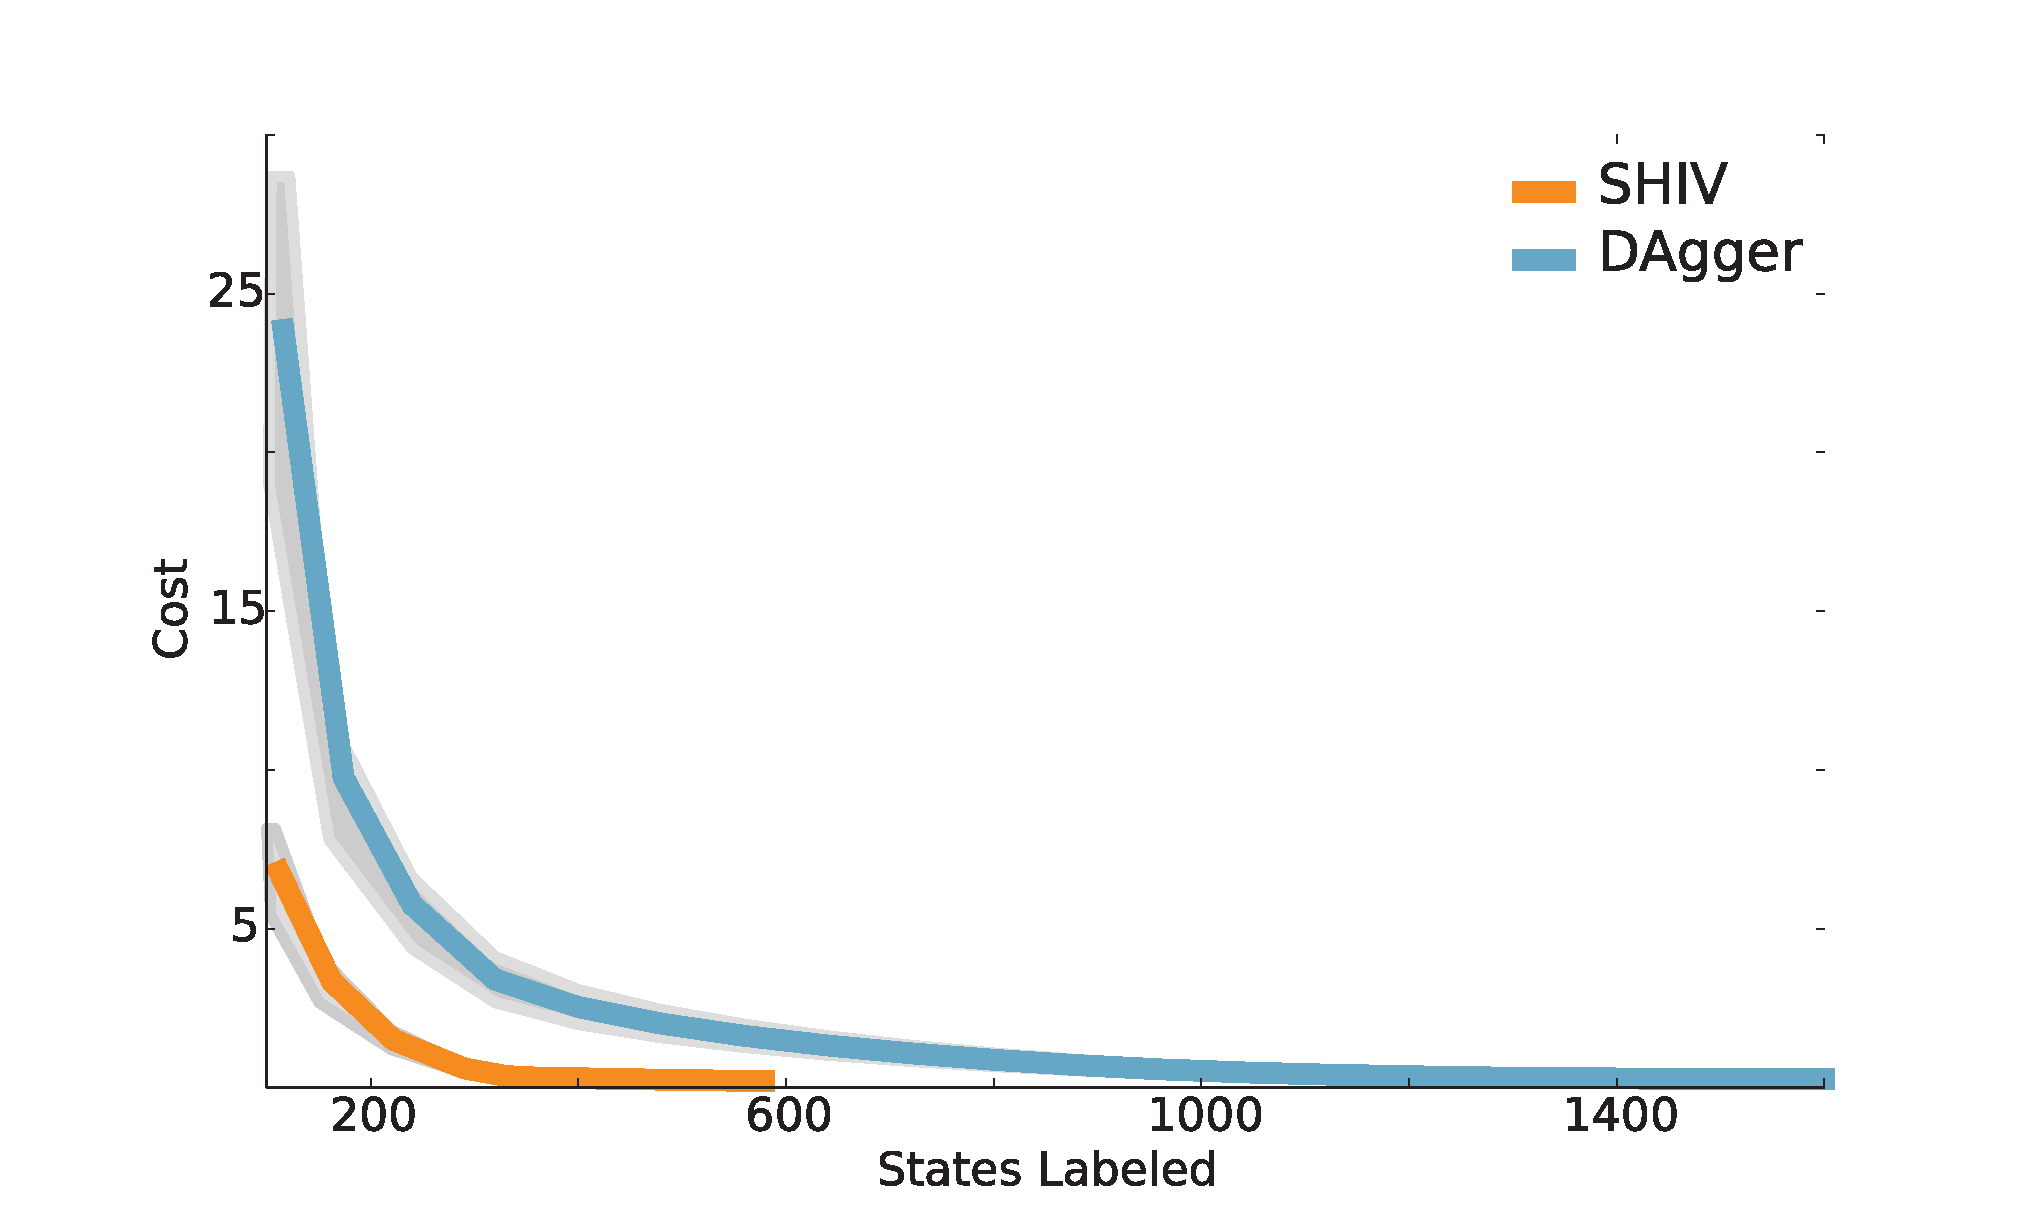
\includegraphics[width=\columnwidth, height=6cm]{figures/needle_insertion_results.eps}
\caption{We compare performance in terms of minimization of the underlying cost function $c(\bx,\bu)$, which is euclidean distance between translation in centimeters. In Fig. \ref{fig:car_cost}, we plot the performance of DAgger and SHIV without the modification.  Initial results, which are run for 20 iterations each and are averaged over 40 different initial starting positions, shown in Fig. \ref{fig:car_cost} suggest an $67\%$ reduction in the number of queries needed for SHIV compared to DAgger,}
\vspace*{-10pt}
\label{fig:needle}
\end{figure}



\section{Discussions and Future Work}
SHIV currently provides a way to apply active learning to online imitation learning, however its use of level set estimation of the underlying distribution introduces several hyper parameters. As Fig. shown these can significantly effect performance if not tuned correctly. Future work will look at using cross validation on a hold out set of data to more effectively tune parameters. 

Another potential issue is that each iteration of SHIV requires solving a quadratic program with the Gram matrix. As we scale to harder tasks that require significantly more data, this can become problematic. Future work will look at using techniques like PCA and random feature projections to scale efficiently \todo{cite something}. 

Lastly, our approach is promising in simulation. However we need to evaluate how our active learning method will work on a real robot with noisy sensor observations. Future work will be doing the grasping in clutter experiments on an actual robot. 

\section{Acknowledgments} 
This work is supported in part by the U.S. National Science Foundation under Award IIS-1227536 and NSF-Graduate Research Fellowship.. 
We thank UC Berkeley and our colleagues who gave feedback and suggestions, in particular Sanjay Krishnan, Siddarth Sen, Steve McKinley, Sachin Patil and Sergey Levine.




\bibliographystyle{IEEEtranS}
\bibliography{references}



\end{document}
